\documentclass[12pt,a4paper]{article}

\usepackage[a4paper,text={16.5cm,25.2cm},centering, margin=1in]{geometry}

\usepackage[scale=0.95]{FiraMono}
\usepackage[utf8]{inputenc}
\usepackage[T1]{fontenc}
\usepackage{mathpazo}

\usepackage{amssymb,amsmath}
\usepackage{bm}
\usepackage{graphicx}
\usepackage{microtype}
\usepackage{hyperref}
\setlength{\parindent}{0pt}
\setlength{\parskip}{1.2ex}

\usepackage{fvextra}
\DefineVerbatimEnvironment{Highlighting}{Verbatim}{breaklines,commandchars=\\\{\}}

\setcounter{secnumdepth}{0}

\hypersetup
       {   pdfauthor = { Akanksha Srivastava (as2752) },
           pdftitle={ BEE 4750/5750 Homework 4 },
           colorlinks=TRUE,
           linkcolor=black,
           citecolor=blue,
           urlcolor=blue
       }

\title{ BEE 4750/5750 Homework 4 }

\author{ Akanksha Srivastava (as2752) }

\date{ 2022-10-25 }

\usepackage{upquote}
\usepackage{listings}
\usepackage{xcolor}
\lstset{
    basicstyle=\ttfamily\footnotesize,
    upquote=true,
    breaklines=true,
    breakindent=0pt,
    keepspaces=true,
    showspaces=false,
    columns=fullflexible,
    showtabs=false,
    showstringspaces=false,
    escapeinside={(*@}{@*)},
    extendedchars=true,
}
\newcommand{\HLJLt}[1]{#1}
\newcommand{\HLJLw}[1]{#1}
\newcommand{\HLJLe}[1]{#1}
\newcommand{\HLJLeB}[1]{#1}
\newcommand{\HLJLo}[1]{#1}
\newcommand{\HLJLk}[1]{\textcolor[RGB]{148,91,176}{\textbf{#1}}}
\newcommand{\HLJLkc}[1]{\textcolor[RGB]{59,151,46}{\textit{#1}}}
\newcommand{\HLJLkd}[1]{\textcolor[RGB]{214,102,97}{\textit{#1}}}
\newcommand{\HLJLkn}[1]{\textcolor[RGB]{148,91,176}{\textbf{#1}}}
\newcommand{\HLJLkp}[1]{\textcolor[RGB]{148,91,176}{\textbf{#1}}}
\newcommand{\HLJLkr}[1]{\textcolor[RGB]{148,91,176}{\textbf{#1}}}
\newcommand{\HLJLkt}[1]{\textcolor[RGB]{148,91,176}{\textbf{#1}}}
\newcommand{\HLJLn}[1]{#1}
\newcommand{\HLJLna}[1]{#1}
\newcommand{\HLJLnb}[1]{#1}
\newcommand{\HLJLnbp}[1]{#1}
\newcommand{\HLJLnc}[1]{#1}
\newcommand{\HLJLncB}[1]{#1}
\newcommand{\HLJLnd}[1]{\textcolor[RGB]{214,102,97}{#1}}
\newcommand{\HLJLne}[1]{#1}
\newcommand{\HLJLneB}[1]{#1}
\newcommand{\HLJLnf}[1]{\textcolor[RGB]{66,102,213}{#1}}
\newcommand{\HLJLnfm}[1]{\textcolor[RGB]{66,102,213}{#1}}
\newcommand{\HLJLnp}[1]{#1}
\newcommand{\HLJLnl}[1]{#1}
\newcommand{\HLJLnn}[1]{#1}
\newcommand{\HLJLno}[1]{#1}
\newcommand{\HLJLnt}[1]{#1}
\newcommand{\HLJLnv}[1]{#1}
\newcommand{\HLJLnvc}[1]{#1}
\newcommand{\HLJLnvg}[1]{#1}
\newcommand{\HLJLnvi}[1]{#1}
\newcommand{\HLJLnvm}[1]{#1}
\newcommand{\HLJLl}[1]{#1}
\newcommand{\HLJLld}[1]{\textcolor[RGB]{148,91,176}{\textit{#1}}}
\newcommand{\HLJLs}[1]{\textcolor[RGB]{201,61,57}{#1}}
\newcommand{\HLJLsa}[1]{\textcolor[RGB]{201,61,57}{#1}}
\newcommand{\HLJLsb}[1]{\textcolor[RGB]{201,61,57}{#1}}
\newcommand{\HLJLsc}[1]{\textcolor[RGB]{201,61,57}{#1}}
\newcommand{\HLJLsd}[1]{\textcolor[RGB]{201,61,57}{#1}}
\newcommand{\HLJLsdB}[1]{\textcolor[RGB]{201,61,57}{#1}}
\newcommand{\HLJLsdC}[1]{\textcolor[RGB]{201,61,57}{#1}}
\newcommand{\HLJLse}[1]{\textcolor[RGB]{59,151,46}{#1}}
\newcommand{\HLJLsh}[1]{\textcolor[RGB]{201,61,57}{#1}}
\newcommand{\HLJLsi}[1]{#1}
\newcommand{\HLJLso}[1]{\textcolor[RGB]{201,61,57}{#1}}
\newcommand{\HLJLsr}[1]{\textcolor[RGB]{201,61,57}{#1}}
\newcommand{\HLJLss}[1]{\textcolor[RGB]{201,61,57}{#1}}
\newcommand{\HLJLssB}[1]{\textcolor[RGB]{201,61,57}{#1}}
\newcommand{\HLJLnB}[1]{\textcolor[RGB]{59,151,46}{#1}}
\newcommand{\HLJLnbB}[1]{\textcolor[RGB]{59,151,46}{#1}}
\newcommand{\HLJLnfB}[1]{\textcolor[RGB]{59,151,46}{#1}}
\newcommand{\HLJLnh}[1]{\textcolor[RGB]{59,151,46}{#1}}
\newcommand{\HLJLni}[1]{\textcolor[RGB]{59,151,46}{#1}}
\newcommand{\HLJLnil}[1]{\textcolor[RGB]{59,151,46}{#1}}
\newcommand{\HLJLnoB}[1]{\textcolor[RGB]{59,151,46}{#1}}
\newcommand{\HLJLoB}[1]{\textcolor[RGB]{102,102,102}{\textbf{#1}}}
\newcommand{\HLJLow}[1]{\textcolor[RGB]{102,102,102}{\textbf{#1}}}
\newcommand{\HLJLp}[1]{#1}
\newcommand{\HLJLc}[1]{\textcolor[RGB]{153,153,119}{\textit{#1}}}
\newcommand{\HLJLch}[1]{\textcolor[RGB]{153,153,119}{\textit{#1}}}
\newcommand{\HLJLcm}[1]{\textcolor[RGB]{153,153,119}{\textit{#1}}}
\newcommand{\HLJLcp}[1]{\textcolor[RGB]{153,153,119}{\textit{#1}}}
\newcommand{\HLJLcpB}[1]{\textcolor[RGB]{153,153,119}{\textit{#1}}}
\newcommand{\HLJLcs}[1]{\textcolor[RGB]{153,153,119}{\textit{#1}}}
\newcommand{\HLJLcsB}[1]{\textcolor[RGB]{153,153,119}{\textit{#1}}}
\newcommand{\HLJLg}[1]{#1}
\newcommand{\HLJLgd}[1]{#1}
\newcommand{\HLJLge}[1]{#1}
\newcommand{\HLJLgeB}[1]{#1}
\newcommand{\HLJLgh}[1]{#1}
\newcommand{\HLJLgi}[1]{#1}
\newcommand{\HLJLgo}[1]{#1}
\newcommand{\HLJLgp}[1]{#1}
\newcommand{\HLJLgs}[1]{#1}
\newcommand{\HLJLgsB}[1]{#1}
\newcommand{\HLJLgt}[1]{#1}


\begin{document}

\maketitle

%  This setups the environment and installs packages, but doesn't appear in the generated document 
%  You shouldn't need to modify this 


\section{Problem 1}
Before tackling individual components, the given information has been entered in Julia for reference:


\begin{lstlisting}
(*@\HLJLcs{{\#}Facility}@*) (*@\HLJLcs{Information}@*)
(*@\HLJLn{facilities}@*) (*@\HLJLoB{=}@*) (*@\HLJLp{[}@*)(*@\HLJLs{"{}WTE"{}}@*)(*@\HLJLp{,}@*) (*@\HLJLs{"{}MRF"{}}@*)(*@\HLJLp{,}@*) (*@\HLJLs{"{}LF"{}}@*)(*@\HLJLp{];}@*) (*@\HLJLcs{{\#}facility}@*) (*@\HLJLcs{types}@*)
(*@\HLJLn{capacities}@*) (*@\HLJLoB{=}@*) (*@\HLJLp{[}@*)(*@\HLJLni{150}@*)(*@\HLJLp{,}@*) (*@\HLJLni{350}@*)(*@\HLJLp{,}@*) (*@\HLJLni{200}@*)(*@\HLJLp{];}@*) (*@\HLJLcs{{\#}Mg/day}@*)
(*@\HLJLn{costs{\_}fixed}@*) (*@\HLJLoB{=}@*) (*@\HLJLp{[}@*)(*@\HLJLni{2500}@*)(*@\HLJLp{,}@*) (*@\HLJLni{1500}@*)(*@\HLJLp{,}@*) (*@\HLJLni{2000}@*)(*@\HLJLp{];}@*) (*@\HLJLcs{{\#}dollars/day}@*)
(*@\HLJLn{tipping{\_}fees}@*) (*@\HLJLoB{=}@*) (*@\HLJLp{[}@*)(*@\HLJLni{60}@*)(*@\HLJLp{,}@*) (*@\HLJLni{7}@*)(*@\HLJLp{,}@*) (*@\HLJLni{50}@*)(*@\HLJLp{];}@*) (*@\HLJLcs{{\#}dollars/Mg}@*)
(*@\HLJLn{costs{\_}recycling}@*) (*@\HLJLoB{=}@*) (*@\HLJLp{[}@*)(*@\HLJLni{0}@*)(*@\HLJLp{,}@*) (*@\HLJLni{45}@*)(*@\HLJLp{,}@*) (*@\HLJLni{0}@*)(*@\HLJLp{];}@*) (*@\HLJLcs{{\#}dollars/Mg}@*) (*@\HLJLcs{recycled}@*)

(*@\HLJLcs{{\#}Relative}@*) (*@\HLJLcs{Distances}@*)
(*@\HLJLn{distance{\_}city1}@*) (*@\HLJLoB{=}@*) (*@\HLJLp{[}@*)(*@\HLJLni{15}@*)(*@\HLJLp{,}@*) (*@\HLJLni{5}@*)(*@\HLJLp{,}@*) (*@\HLJLni{30}@*)(*@\HLJLp{];}@*) (*@\HLJLcs{{\#}km}@*)
(*@\HLJLn{distance{\_}city2}@*) (*@\HLJLoB{=}@*) (*@\HLJLp{[}@*)(*@\HLJLni{10}@*)(*@\HLJLp{,}@*) (*@\HLJLni{15}@*)(*@\HLJLp{,}@*) (*@\HLJLni{25}@*)(*@\HLJLp{];}@*) (*@\HLJLcs{{\#}km}@*)
(*@\HLJLn{distance{\_}WTE}@*) (*@\HLJLoB{=}@*) (*@\HLJLp{[}@*)(*@\HLJLni{0}@*)(*@\HLJLp{,}@*) (*@\HLJLni{15}@*)(*@\HLJLp{,}@*) (*@\HLJLni{18}@*)(*@\HLJLp{];}@*) (*@\HLJLcs{{\#}km}@*)
(*@\HLJLn{distance{\_}MRF}@*) (*@\HLJLoB{=}@*) (*@\HLJLp{[}@*)(*@\HLJLni{15}@*)(*@\HLJLp{,}@*) (*@\HLJLni{0}@*)(*@\HLJLp{,}@*) (*@\HLJLni{32}@*)(*@\HLJLp{];}@*) (*@\HLJLcs{{\#}km}@*)
(*@\HLJLn{distance{\_}LF}@*) (*@\HLJLoB{=}@*) (*@\HLJLp{[}@*)(*@\HLJLni{18}@*)(*@\HLJLp{,}@*) (*@\HLJLni{32}@*)(*@\HLJLp{,}@*) (*@\HLJLni{0}@*)(*@\HLJLp{];}@*) (*@\HLJLcs{{\#}km}@*)

(*@\HLJLcs{{\#}Transportation}@*) (*@\HLJLcs{Costs}@*)
(*@\HLJLn{cost{\_}transport}@*) (*@\HLJLoB{=}@*) (*@\HLJLnfB{1.5}@*)(*@\HLJLp{;}@*) (*@\HLJLcs{{\#}dollars/Mg/km}@*)

(*@\HLJLcs{{\#}Waste}@*) (*@\HLJLcs{Production}@*)
(*@\HLJLn{solid{\_}waste}@*) (*@\HLJLoB{=}@*) (*@\HLJLp{[}@*)(*@\HLJLni{100}@*)(*@\HLJLp{,}@*) (*@\HLJLni{170}@*)(*@\HLJLp{];}@*) (*@\HLJLcs{{\#}Mg/day}@*)

(*@\HLJLcs{{\#}Waste}@*) (*@\HLJLcs{Composition}@*) (*@\HLJLcs{and}@*) (*@\HLJLcs{Properties}@*)
(*@\HLJLn{components}@*) (*@\HLJLoB{=}@*) (*@\HLJLp{[}@*)(*@\HLJLs{"{}Food"{}}@*)(*@\HLJLp{,}@*)(*@\HLJLs{"{}Paper"{}}@*)(*@\HLJLp{,}@*)(*@\HLJLs{"{}Plastic"{}}@*)(*@\HLJLp{,}@*)(*@\HLJLs{"{}Textile"{}}@*)(*@\HLJLp{,}@*)(*@\HLJLs{"{}Rubber"{}}@*)(*@\HLJLp{,}@*)(*@\HLJLs{"{}Wood"{}}@*)(*@\HLJLp{,}@*)(*@\HLJLs{"{}Yard"{}}@*)(*@\HLJLp{,}@*)(*@\HLJLs{"{}Glass"{}}@*)(*@\HLJLp{,}@*)(*@\HLJLs{"{}Fe"{}}@*)(*@\HLJLp{,}@*)(*@\HLJLs{"{}Al"{}}@*)(*@\HLJLp{,}@*)(*@\HLJLs{"{}Metal"{}}@*)(*@\HLJLp{,}@*)(*@\HLJLs{"{}Misc"{}}@*)(*@\HLJLp{];}@*)
(*@\HLJLn{mass{\_}percent}@*) (*@\HLJLoB{=}@*) (*@\HLJLp{[}@*)(*@\HLJLni{15}@*)(*@\HLJLp{,}@*) (*@\HLJLni{40}@*)(*@\HLJLp{,}@*) (*@\HLJLni{5}@*)(*@\HLJLp{,}@*) (*@\HLJLni{3}@*)(*@\HLJLp{,}@*) (*@\HLJLni{2}@*)(*@\HLJLp{,}@*) (*@\HLJLni{5}@*)(*@\HLJLp{,}@*) (*@\HLJLni{18}@*)(*@\HLJLp{,}@*) (*@\HLJLni{4}@*)(*@\HLJLp{,}@*) (*@\HLJLni{2}@*)(*@\HLJLp{,}@*) (*@\HLJLni{2}@*)(*@\HLJLp{,}@*) (*@\HLJLni{1}@*)(*@\HLJLp{,}@*) (*@\HLJLni{3}@*)(*@\HLJLp{];}@*)
(*@\HLJLn{ash{\_}percent}@*) (*@\HLJLoB{=}@*) (*@\HLJLp{[}@*)(*@\HLJLni{8}@*)(*@\HLJLp{,}@*) (*@\HLJLni{7}@*)(*@\HLJLp{,}@*) (*@\HLJLni{5}@*)(*@\HLJLp{,}@*) (*@\HLJLni{10}@*)(*@\HLJLp{,}@*) (*@\HLJLni{15}@*)(*@\HLJLp{,}@*) (*@\HLJLni{2}@*)(*@\HLJLp{,}@*) (*@\HLJLni{2}@*)(*@\HLJLp{,}@*) (*@\HLJLni{100}@*)(*@\HLJLp{,}@*) (*@\HLJLni{100}@*)(*@\HLJLp{,}@*) (*@\HLJLni{100}@*)(*@\HLJLp{,}@*) (*@\HLJLni{100}@*)(*@\HLJLp{,}@*) (*@\HLJLni{70}@*)(*@\HLJLp{];}@*)
(*@\HLJLn{rec{\_}percent}@*) (*@\HLJLoB{=}@*) (*@\HLJLp{[}@*)(*@\HLJLni{0}@*)(*@\HLJLp{,}@*) (*@\HLJLni{55}@*)(*@\HLJLp{,}@*) (*@\HLJLni{15}@*)(*@\HLJLp{,}@*) (*@\HLJLni{10}@*)(*@\HLJLp{,}@*) (*@\HLJLni{0}@*)(*@\HLJLp{,}@*) (*@\HLJLni{30}@*)(*@\HLJLp{,}@*) (*@\HLJLni{40}@*)(*@\HLJLp{,}@*) (*@\HLJLni{60}@*)(*@\HLJLp{,}@*) (*@\HLJLni{75}@*)(*@\HLJLp{,}@*) (*@\HLJLni{80}@*)(*@\HLJLp{,}@*) (*@\HLJLni{50}@*)(*@\HLJLp{,}@*) (*@\HLJLni{0}@*)(*@\HLJLp{];}@*)
\end{lstlisting}


\subsection{Problem 1.1}
The following Julia code calculates the overall recycling and ash fractions for the waste produced by each city:


\begin{lstlisting}
(*@\HLJLn{rec{\_}frac}@*) (*@\HLJLoB{=}@*) (*@\HLJLn{mass{\_}percent}@*)(*@\HLJLoB{{\textquotesingle}*}@*)(*@\HLJLn{rec{\_}percent}@*) (*@\HLJLoB{/}@*) (*@\HLJLni{10000}@*)(*@\HLJLp{;}@*)
(*@\HLJLn{ash{\_}frac}@*) (*@\HLJLoB{=}@*) (*@\HLJLn{mass{\_}percent}@*)(*@\HLJLoB{{\textquotesingle}*}@*)(*@\HLJLn{ash{\_}percent}@*) (*@\HLJLoB{/}@*) (*@\HLJLni{10000}@*)(*@\HLJLp{;}@*)
\end{lstlisting}


This gives us a recycling rate of 37.75\% and an ash fraction of 16.41\%.

\subsection{Problem 1.2}
The decision variables for this optimization problem are:

\begin{itemize}
\item[1. ] Waste transported from city i to disposal j in Mg/day, $W_{ij}$


\item[2. ] Residual waste transported from disposal k to disposal j in Mg/day, $R_{kj}$


\item[3. ] Operational status of disposal j (a binary variable), $Y_j$

\end{itemize}
\subsection{Problem 1.3}
The objective function will be to minimize the sum of disposal costs and transportation costs:

\[
Cost = \sum_i\sum_j a_{ij}l_{ij}W_{ij} + \sum_j[c_jY_j+\sum_ib_jW_{ij}]
\]
where $a_{ij}$ is the cost of transporting waste from source i to disposal j in dollars/Mg-km,  $l_{ij}$ is the distance between sources i and disposal j in km,  $c_j$ is the fixed cost of operating disposal j in dollars/day, and  $b_j$ is the variable cost of disposing waste at disposal j in dollars/Mg.

For the specifics of this problem, this translates to:

\begin{itemize}
\item[1. ] Waste-to-Energy: $2500Y_1 + 60(W_{11}+W_{21}+R_{21})$


\item[2. ] Material Recovery: $1500Y_2 + 7(W_{21}+W_{22})+0.3775(45)(W_{12}+W_{22})$


\item[3. ] Landfill: $2000Y_3 + 50(W_{13}+W_{23}+R_{13}+R_{23})$


\item[4. ] Transportation: $1.5[15W_{11}+5W_{12}+30W_{13}+10W_{21}+15W_{22}+25W_{23}+18R_{13}+15R_{21}+32R_{23}]$

\end{itemize}
Then the total cost is: $2500Y_1 + 1500Y_2 + 2000Y_3 + 82.5W_{11} + 31.4875W_{12} + 95W_{13} + 75W_{21} + 46.4875W_{22} + 87.5W_{23} + 77R_{13} + 82.5R_{21} + 98R_{23}$

\subsection{Problem 1.4}
Constraints can be organized into city mass balance, capacity mass balance, recycling rate and residual ash constraints, and committment and nonnegativity constraints.

City Mass Balance Constraints: The sum of waste sent to each facility must equal the waste produced by each city.

\begin{itemize}
\item City 1: $W_{11}+W_{12}+W_{13}=100$


\item City 2: $W_{21}+W_{22}+W_{23}=170$

\end{itemize}
Capacity Mass Balance Constraints: The total weights sent to each facility must not exceed their capacities.

\begin{itemize}
\item WTE: $W_{11}+W_{21}+R_{21} \leq 150$


\item MRF: $W_{12}+W_{22} \leq 350$


\item LF: $W_{13}+W_{23}+R_{23}+R_{13} \leq 200$

\end{itemize}
Recycling Rate and Residual Ash Constraints: The waste sent from the WTE must be equal to the ash weight produced, and the weight  sent from the MRF must be the non-recycled waste that entered the facility.

\begin{itemize}
\item Residual Ash: $R_{13} = 0.1641(W_{11}+W_{21}+R_{21})$


\item Recycling Rate: $R_{21}+R_{23}=(1-0.3775)(W_{12}+W_{22})$

\end{itemize}
Commitment and Non-Negativity: Defining the binary variables and making all waste streams nonnegative

\begin{itemize}
\item If $W_{11}+W_{21}+R_{21}=0$, $Y_1=0$, else $Y_1=1$


\item If $W_{21}+W_{22}=0$, $Y_1=0$, else $Y_1=1$


\item The landfill must be on: $Y_3=1$


\item Nonnegativity: $W_{ij},R_{ij} \geq 0$

\end{itemize}
\subsection{Problem 1.5}

\begin{lstlisting}
(*@\HLJLk{using}@*) (*@\HLJLn{JuMP}@*)
(*@\HLJLk{using}@*) (*@\HLJLn{Cbc}@*)

(*@\HLJLn{waste}@*) (*@\HLJLoB{=}@*) (*@\HLJLnf{Model}@*)(*@\HLJLp{(}@*)(*@\HLJLn{Cbc}@*)(*@\HLJLoB{.}@*)(*@\HLJLn{Optimizer}@*)(*@\HLJLp{)}@*)
(*@\HLJLn{I}@*) (*@\HLJLoB{=}@*) (*@\HLJLni{1}@*)(*@\HLJLoB{:}@*)(*@\HLJLni{2}@*)(*@\HLJLp{;}@*) (*@\HLJLcs{{\#}number}@*) (*@\HLJLcs{of}@*) (*@\HLJLcs{cities}@*)
(*@\HLJLn{J}@*) (*@\HLJLoB{=}@*) (*@\HLJLni{1}@*)(*@\HLJLoB{:}@*)(*@\HLJLni{3}@*)(*@\HLJLp{;}@*) (*@\HLJLcs{{\#}number}@*) (*@\HLJLcs{of}@*) (*@\HLJLcs{disposal}@*) (*@\HLJLcs{sites}@*)

(*@\HLJLnd{@variable}@*)(*@\HLJLp{(}@*)(*@\HLJLn{waste}@*)(*@\HLJLp{,}@*) (*@\HLJLn{W}@*)(*@\HLJLp{[}@*)(*@\HLJLn{i}@*) (*@\HLJLkp{in}@*) (*@\HLJLn{I}@*)(*@\HLJLp{,}@*) (*@\HLJLn{j}@*) (*@\HLJLkp{in}@*) (*@\HLJLn{J}@*)(*@\HLJLp{]}@*) (*@\HLJLoB{>=}@*) (*@\HLJLni{0}@*)(*@\HLJLp{);}@*)
(*@\HLJLnd{@variable}@*)(*@\HLJLp{(}@*)(*@\HLJLn{waste}@*)(*@\HLJLp{,}@*) (*@\HLJLn{R}@*)(*@\HLJLp{[}@*)(*@\HLJLn{k}@*) (*@\HLJLkp{in}@*) (*@\HLJLn{J}@*)(*@\HLJLp{,}@*) (*@\HLJLn{j}@*) (*@\HLJLkp{in}@*) (*@\HLJLn{J}@*)(*@\HLJLp{]}@*) (*@\HLJLoB{>=}@*) (*@\HLJLni{0}@*)(*@\HLJLp{);}@*)
(*@\HLJLnd{@variable}@*)(*@\HLJLp{(}@*)(*@\HLJLn{waste}@*)(*@\HLJLp{,}@*) (*@\HLJLn{Y}@*)(*@\HLJLp{[}@*)(*@\HLJLn{j}@*) (*@\HLJLkp{in}@*) (*@\HLJLn{J}@*)(*@\HLJLp{],}@*) (*@\HLJLn{Bin}@*)(*@\HLJLp{);}@*)
(*@\HLJLnd{@objective}@*)(*@\HLJLp{(}@*)(*@\HLJLn{waste}@*)(*@\HLJLp{,}@*) (*@\HLJLn{Min}@*)(*@\HLJLp{,}@*) (*@\HLJLnf{sum}@*)(*@\HLJLp{([}@*)(*@\HLJLnfB{82.5}@*) (*@\HLJLnfB{31.4875}@*) (*@\HLJLni{95}@*)(*@\HLJLp{;}@*) (*@\HLJLni{75}@*) (*@\HLJLnfB{46.4875}@*) (*@\HLJLnfB{87.5}@*)(*@\HLJLp{]}@*)(*@\HLJLoB{.*}@*)(*@\HLJLn{W}@*)(*@\HLJLp{)}@*)(*@\HLJLoB{+}@*)(*@\HLJLnf{sum}@*)(*@\HLJLp{([}@*)(*@\HLJLni{0}@*) (*@\HLJLni{0}@*) (*@\HLJLni{77}@*)(*@\HLJLp{;}@*) (*@\HLJLnfB{82.5}@*) (*@\HLJLni{0}@*) (*@\HLJLni{98}@*)(*@\HLJLp{;}@*) (*@\HLJLni{0}@*) (*@\HLJLni{0}@*) (*@\HLJLni{0}@*)(*@\HLJLp{]}@*)(*@\HLJLoB{.*}@*)(*@\HLJLn{R}@*)(*@\HLJLp{)}@*) (*@\HLJLoB{+}@*) (*@\HLJLnf{sum}@*)(*@\HLJLp{(}@*)(*@\HLJLn{costs{\_}fixed}@*) (*@\HLJLoB{.*}@*) (*@\HLJLn{Y}@*)(*@\HLJLp{));}@*)

(*@\HLJLcs{{\#}}@*) (*@\HLJLcs{mass-balance}@*)
(*@\HLJLnd{@constraint}@*)(*@\HLJLp{(}@*)(*@\HLJLn{waste}@*)(*@\HLJLp{,}@*) (*@\HLJLn{city}@*)(*@\HLJLp{[}@*)(*@\HLJLn{i}@*) (*@\HLJLkp{in}@*) (*@\HLJLn{I}@*)(*@\HLJLp{],}@*) (*@\HLJLnf{sum}@*)(*@\HLJLp{(}@*)(*@\HLJLn{W}@*)(*@\HLJLp{[}@*)(*@\HLJLn{i}@*)(*@\HLJLp{,}@*)(*@\HLJLoB{:}@*)(*@\HLJLp{])}@*) (*@\HLJLoB{==}@*) (*@\HLJLn{solid{\_}waste}@*)(*@\HLJLp{[}@*)(*@\HLJLn{i}@*)(*@\HLJLp{]);}@*)
(*@\HLJLnd{@constraint}@*)(*@\HLJLp{(}@*)(*@\HLJLn{waste}@*)(*@\HLJLp{,}@*) (*@\HLJLn{wte}@*)(*@\HLJLp{,}@*) (*@\HLJLn{W}@*)(*@\HLJLp{[}@*)(*@\HLJLni{1}@*)(*@\HLJLp{,}@*)(*@\HLJLni{1}@*)(*@\HLJLp{]}@*) (*@\HLJLoB{+}@*) (*@\HLJLn{W}@*)(*@\HLJLp{[}@*)(*@\HLJLni{2}@*)(*@\HLJLp{,}@*)(*@\HLJLni{1}@*)(*@\HLJLp{]}@*) (*@\HLJLoB{+}@*) (*@\HLJLn{R}@*)(*@\HLJLp{[}@*)(*@\HLJLni{2}@*)(*@\HLJLp{,}@*)(*@\HLJLni{1}@*)(*@\HLJLp{]}@*) (*@\HLJLoB{<=}@*) (*@\HLJLn{capacities}@*)(*@\HLJLp{[}@*)(*@\HLJLni{1}@*)(*@\HLJLp{]);}@*)
(*@\HLJLnd{@constraint}@*)(*@\HLJLp{(}@*)(*@\HLJLn{waste}@*)(*@\HLJLp{,}@*) (*@\HLJLn{mrf}@*)(*@\HLJLp{,}@*) (*@\HLJLn{W}@*)(*@\HLJLp{[}@*)(*@\HLJLni{1}@*)(*@\HLJLp{,}@*)(*@\HLJLni{2}@*)(*@\HLJLp{]}@*) (*@\HLJLoB{+}@*) (*@\HLJLn{W}@*)(*@\HLJLp{[}@*)(*@\HLJLni{2}@*)(*@\HLJLp{,}@*)(*@\HLJLni{2}@*)(*@\HLJLp{]}@*)  (*@\HLJLoB{<=}@*) (*@\HLJLn{capacities}@*)(*@\HLJLp{[}@*)(*@\HLJLni{2}@*)(*@\HLJLp{]);}@*)
(*@\HLJLnd{@constraint}@*)(*@\HLJLp{(}@*)(*@\HLJLn{waste}@*)(*@\HLJLp{,}@*) (*@\HLJLn{lf}@*)(*@\HLJLp{,}@*) (*@\HLJLn{W}@*)(*@\HLJLp{[}@*)(*@\HLJLni{1}@*)(*@\HLJLp{,}@*)(*@\HLJLni{3}@*)(*@\HLJLp{]}@*) (*@\HLJLoB{+}@*) (*@\HLJLn{W}@*)(*@\HLJLp{[}@*)(*@\HLJLni{2}@*)(*@\HLJLp{,}@*)(*@\HLJLni{3}@*)(*@\HLJLp{]}@*) (*@\HLJLoB{+}@*) (*@\HLJLn{R}@*)(*@\HLJLp{[}@*)(*@\HLJLni{2}@*)(*@\HLJLp{,}@*)(*@\HLJLni{3}@*)(*@\HLJLp{]}@*) (*@\HLJLoB{+}@*) (*@\HLJLn{R}@*)(*@\HLJLp{[}@*)(*@\HLJLni{1}@*)(*@\HLJLp{,}@*)(*@\HLJLni{3}@*)(*@\HLJLp{]}@*) (*@\HLJLoB{<=}@*) (*@\HLJLn{capacities}@*)(*@\HLJLp{[}@*)(*@\HLJLni{3}@*)(*@\HLJLp{]);}@*)

(*@\HLJLcs{{\#}}@*) (*@\HLJLcs{residuals}@*)
(*@\HLJLnd{@constraint}@*)(*@\HLJLp{(}@*)(*@\HLJLn{waste}@*)(*@\HLJLp{,}@*) (*@\HLJLn{resid1}@*)(*@\HLJLp{,}@*) (*@\HLJLn{R}@*)(*@\HLJLp{[}@*)(*@\HLJLni{1}@*)(*@\HLJLp{,}@*)(*@\HLJLni{3}@*)(*@\HLJLp{]}@*) (*@\HLJLoB{==}@*) (*@\HLJLn{ash{\_}frac}@*) (*@\HLJLoB{.*}@*) (*@\HLJLp{(}@*)(*@\HLJLn{W}@*)(*@\HLJLp{[}@*)(*@\HLJLni{1}@*)(*@\HLJLp{,}@*)(*@\HLJLni{1}@*)(*@\HLJLp{]}@*) (*@\HLJLoB{+}@*) (*@\HLJLn{W}@*)(*@\HLJLp{[}@*)(*@\HLJLni{2}@*)(*@\HLJLp{,}@*)(*@\HLJLni{1}@*)(*@\HLJLp{]}@*) (*@\HLJLoB{+}@*) (*@\HLJLn{R}@*)(*@\HLJLp{[}@*)(*@\HLJLni{2}@*)(*@\HLJLp{,}@*)(*@\HLJLni{1}@*)(*@\HLJLp{]));}@*)
(*@\HLJLnd{@constraint}@*)(*@\HLJLp{(}@*)(*@\HLJLn{waste}@*)(*@\HLJLp{,}@*) (*@\HLJLn{resid2}@*)(*@\HLJLp{,}@*) (*@\HLJLn{R}@*)(*@\HLJLp{[}@*)(*@\HLJLni{2}@*)(*@\HLJLp{,}@*)(*@\HLJLni{1}@*)(*@\HLJLp{]}@*) (*@\HLJLoB{+}@*) (*@\HLJLn{R}@*)(*@\HLJLp{[}@*)(*@\HLJLni{2}@*)(*@\HLJLp{,}@*)(*@\HLJLni{3}@*)(*@\HLJLp{]}@*) (*@\HLJLoB{==}@*) (*@\HLJLp{(}@*)(*@\HLJLni{1}@*)(*@\HLJLoB{-}@*)(*@\HLJLn{rec{\_}frac}@*)(*@\HLJLp{)}@*) (*@\HLJLoB{.*}@*) (*@\HLJLp{(}@*)(*@\HLJLn{W}@*)(*@\HLJLp{[}@*)(*@\HLJLni{1}@*)(*@\HLJLp{,}@*)(*@\HLJLni{2}@*)(*@\HLJLp{]}@*) (*@\HLJLoB{+}@*) (*@\HLJLn{W}@*)(*@\HLJLp{[}@*)(*@\HLJLni{2}@*)(*@\HLJLp{,}@*)(*@\HLJLni{2}@*)(*@\HLJLp{]));}@*)
(*@\HLJLnd{@constraint}@*)(*@\HLJLp{(}@*)(*@\HLJLn{waste}@*)(*@\HLJLp{,}@*) (*@\HLJLn{resid3}@*)(*@\HLJLp{,}@*) (*@\HLJLnf{sum}@*)(*@\HLJLp{(}@*)(*@\HLJLn{R}@*)(*@\HLJLp{[}@*)(*@\HLJLni{3}@*)(*@\HLJLp{,}@*)(*@\HLJLoB{:}@*)(*@\HLJLp{])}@*) (*@\HLJLoB{==}@*) (*@\HLJLni{0}@*)(*@\HLJLp{);}@*)
(*@\HLJLnd{@constraint}@*)(*@\HLJLp{(}@*)(*@\HLJLn{waste}@*)(*@\HLJLp{,}@*) (*@\HLJLn{noresiddiag}@*)(*@\HLJLp{,}@*) (*@\HLJLnf{sum}@*)(*@\HLJLp{(}@*)(*@\HLJLn{R}@*)(*@\HLJLp{[}@*)(*@\HLJLn{i}@*)(*@\HLJLp{,}@*) (*@\HLJLn{i}@*)(*@\HLJLp{]}@*) (*@\HLJLk{for}@*) (*@\HLJLn{i}@*) (*@\HLJLkp{in}@*) (*@\HLJLn{I}@*)(*@\HLJLp{)}@*) (*@\HLJLoB{==}@*) (*@\HLJLni{0}@*)(*@\HLJLp{);}@*)
(*@\HLJLnd{@constraint}@*)(*@\HLJLp{(}@*)(*@\HLJLn{waste}@*)(*@\HLJLp{,}@*) (*@\HLJLn{noresid}@*)(*@\HLJLp{,}@*) (*@\HLJLn{R}@*)(*@\HLJLp{[}@*)(*@\HLJLni{1}@*)(*@\HLJLp{,}@*)(*@\HLJLni{2}@*)(*@\HLJLp{]}@*) (*@\HLJLoB{==}@*) (*@\HLJLni{0}@*)(*@\HLJLp{);}@*)

(*@\HLJLcs{{\#}}@*) (*@\HLJLcs{commitment}@*)
(*@\HLJLnd{@constraint}@*)(*@\HLJLp{(}@*)(*@\HLJLn{waste}@*)(*@\HLJLp{,}@*) (*@\HLJLn{commit1}@*)(*@\HLJLp{,}@*) (*@\HLJLoB{!}@*)(*@\HLJLn{Y}@*)(*@\HLJLp{[}@*)(*@\HLJLni{1}@*)(*@\HLJLp{]}@*) (*@\HLJLoB{=>}@*) (*@\HLJLp{{\{}}@*)(*@\HLJLn{W}@*)(*@\HLJLp{[}@*)(*@\HLJLni{1}@*)(*@\HLJLp{,}@*)(*@\HLJLni{1}@*)(*@\HLJLp{]}@*) (*@\HLJLoB{+}@*) (*@\HLJLn{W}@*)(*@\HLJLp{[}@*)(*@\HLJLni{2}@*)(*@\HLJLp{,}@*)(*@\HLJLni{1}@*)(*@\HLJLp{]}@*) (*@\HLJLoB{+}@*) (*@\HLJLn{R}@*)(*@\HLJLp{[}@*)(*@\HLJLni{2}@*)(*@\HLJLp{,}@*)(*@\HLJLni{1}@*)(*@\HLJLp{]}@*) (*@\HLJLoB{==}@*) (*@\HLJLni{0}@*)(*@\HLJLp{{\}});}@*)
(*@\HLJLnd{@constraint}@*)(*@\HLJLp{(}@*)(*@\HLJLn{waste}@*)(*@\HLJLp{,}@*) (*@\HLJLn{commit2}@*)(*@\HLJLp{,}@*) (*@\HLJLoB{!}@*)(*@\HLJLn{Y}@*)(*@\HLJLp{[}@*)(*@\HLJLni{2}@*)(*@\HLJLp{]}@*) (*@\HLJLoB{=>}@*) (*@\HLJLp{{\{}}@*)(*@\HLJLn{W}@*)(*@\HLJLp{[}@*)(*@\HLJLni{1}@*)(*@\HLJLp{,}@*)(*@\HLJLni{2}@*)(*@\HLJLp{]}@*) (*@\HLJLoB{+}@*) (*@\HLJLn{W}@*)(*@\HLJLp{[}@*)(*@\HLJLni{2}@*)(*@\HLJLp{,}@*)(*@\HLJLni{2}@*)(*@\HLJLp{]}@*) (*@\HLJLoB{==}@*) (*@\HLJLni{0}@*)(*@\HLJLp{{\}});}@*)
(*@\HLJLnd{@constraint}@*)(*@\HLJLp{(}@*)(*@\HLJLn{waste}@*)(*@\HLJLp{,}@*) (*@\HLJLn{commit3}@*)(*@\HLJLp{,}@*) (*@\HLJLn{Y}@*)(*@\HLJLp{[}@*)(*@\HLJLni{3}@*)(*@\HLJLp{]}@*) (*@\HLJLoB{==}@*) (*@\HLJLni{1}@*)(*@\HLJLp{);}@*)

(*@\HLJLnf{optimize!}@*)(*@\HLJLp{(}@*)(*@\HLJLn{waste}@*)(*@\HLJLp{);}@*)
\end{lstlisting}

Welcome to the CBC MILP Solver 
Version: 2.10.5 
Build Date: Dec  4 2021 

command line - Cbc_C_Interface -solve -quit (default strategy 1)
Continuous objective value is 25945.9 - 0.00 seconds
Cgl0003I 0 fixed, 0 tightened bounds, 0 strengthened rows, 2 substitutions
Cgl0003I 0 fixed, 0 tightened bounds, 0 strengthened rows, 2 substitutions
Cgl0003I 0 fixed, 0 tightened bounds, 0 strengthened rows, 2 substitutions
Cgl0003I 0 fixed, 0 tightened bounds, 0 strengthened rows, 2 substitutions
Cgl0003I 0 fixed, 0 tightened bounds, 0 strengthened rows, 2 substitutions
Cgl0003I 0 fixed, 0 tightened bounds, 0 strengthened rows, 2 substitutions
Cgl0003I 0 fixed, 0 tightened bounds, 0 strengthened rows, 2 substitutions
Cgl0003I 0 fixed, 0 tightened bounds, 0 strengthened rows, 2 substitutions
Cgl0003I 0 fixed, 0 tightened bounds, 0 strengthened rows, 2 substitutions
Cgl0004I processed model has 11 rows, 14 columns (4 integer (4 of which binary)) and 34 elements
Cbc0036I Heuristics switched off as 2 branching objects are of wrong type
Cbc0013I At root node, 0 cuts changed objective from 25945.947 to 25945.947 in 1 passes
Cbc0014I Cut generator 0 (Probing) - 0 row cuts average 0.0 elements, 0 column cuts (0 active)  in 0.000 seconds - new frequency is -100
Cbc0014I Cut generator 1 (Gomory) - 0 row cuts average 0.0 elements, 0 column cuts (0 active)  in 0.000 seconds - new frequency is -100
Cbc0014I Cut generator 2 (Knapsack) - 0 row cuts average 0.0 elements, 0 column cuts (0 active)  in 0.000 seconds - new frequency is -100
Cbc0014I Cut generator 3 (Clique) - 0 row cuts average 0.0 elements, 0 column cuts (0 active)  in 0.000 seconds - new frequency is -100
Cbc0014I Cut generator 4 (MixedIntegerRounding2) - 0 row cuts average 0.0 elements, 0 column cuts (0 active)  in 0.000 seconds - new frequency is -100
Cbc0014I Cut generator 5 (FlowCover) - 0 row cuts average 0.0 elements, 0 column cuts (0 active)  in 0.000 seconds - new frequency is -100
Cbc0010I After 0 nodes, 1 on tree, 1e+50 best solution, best possible 25945.947 (0.00 seconds)
Cbc0016I Integer solution of 28886.364 found by strong branching after 2 iterations and 1 nodes (0.00 seconds)
Cbc0001I Search completed - best objective 28886.36379949755, took 2 iterations and 2 nodes (0.01 seconds)
Cbc0032I Strong branching done 8 times (9 iterations), fathomed 2 nodes and fixed 0 variables
Cbc0035I Maximum depth 0, 1 variables fixed on reduced cost
Cuts at root node changed objective from 25945.9 to 25945.9
Probing was tried 1 times and created 0 cuts of which 0 were active after adding rounds of cuts (0.000 seconds)
Gomory was tried 1 times and created 0 cuts of which 0 were active after adding rounds of cuts (0.000 seconds)
Knapsack was tried 1 times and created 0 cuts of which 0 were active after adding rounds of cuts (0.000 seconds)
Clique was tried 1 times and created 0 cuts of which 0 were active after adding rounds of cuts (0.000 seconds)
MixedIntegerRounding2 was tried 1 times and created 0 cuts of which 0 were active after adding rounds of cuts (0.000 seconds)
FlowCover was tried 1 times and created 0 cuts of which 0 were active after adding rounds of cuts (0.000 seconds)
TwoMirCuts was tried 1 times and created 0 cuts of which 0 were active after adding rounds of cuts (0.000 seconds)
ZeroHalf was tried 1 times and created 0 cuts of which 0 were active after adding rounds of cuts (0.000 seconds)
9 bounds tightened after postprocessing


Result - Optimal solution found

Objective value:                28886.36379950
Enumerated nodes:               2
Total iterations:               2
Time (CPU seconds):             0.01
Time (Wallclock seconds):       0.01

Total time (CPU seconds):       0.01   (Wallclock seconds):       0.01



\subsection{Problem 1.6}

\begin{lstlisting}
(*@\HLJLn{min{\_}cost}@*) (*@\HLJLoB{=}@*) (*@\HLJLnf{objective{\_}value}@*)(*@\HLJLp{(}@*)(*@\HLJLn{waste}@*)(*@\HLJLp{);}@*)
(*@\HLJLn{commitments}@*) (*@\HLJLoB{=}@*) (*@\HLJLn{value}@*)(*@\HLJLoB{.}@*)(*@\HLJLp{(}@*)(*@\HLJLn{Y}@*)(*@\HLJLp{);}@*)
(*@\HLJLn{waste{\_}values}@*) (*@\HLJLoB{=}@*) (*@\HLJLn{value}@*)(*@\HLJLoB{.}@*)(*@\HLJLp{(}@*)(*@\HLJLn{W}@*)(*@\HLJLp{);}@*)
(*@\HLJLn{residual{\_}values}@*) (*@\HLJLoB{=}@*) (*@\HLJLn{value}@*)(*@\HLJLoB{.}@*)(*@\HLJLp{(}@*)(*@\HLJLn{R}@*)(*@\HLJLp{);}@*)
\end{lstlisting}


The objective value is 28,886.36 dollars, and the MRF facility will not be used in this scenario.  The following diagram depicts the waste flows from the cities to the facilities. \begin{figure}
\centering
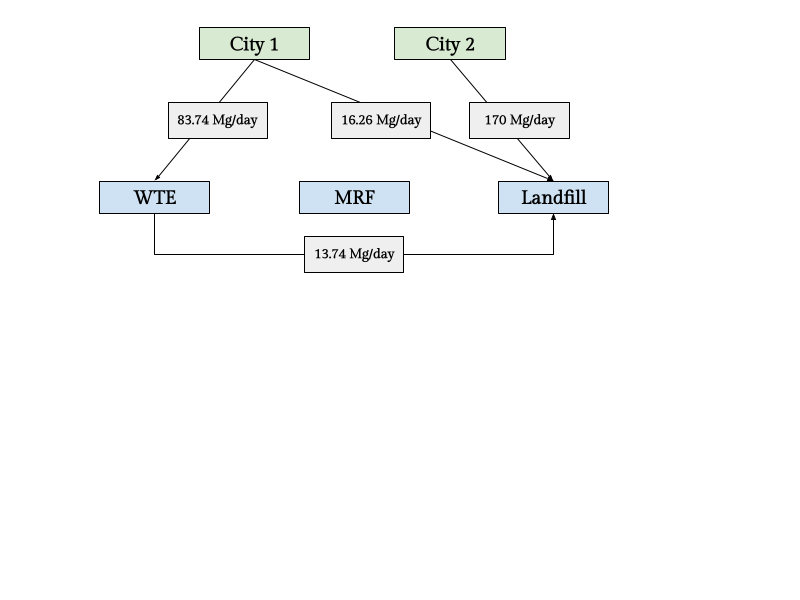
\includegraphics{waste_diagram.png}
\caption{Waste Diagram}
\end{figure}


\section{Problem 2}
\subsection{Problem 2.1}
\subsection{Problem 2.2}
\subsection{Problem 2.3}
\section{References}
\begin{itemize}
\item[1. ] Optimization Setup: Mixed Integer Programming and Waste Management Lecture (10/17)

\end{itemize}


\end{document}